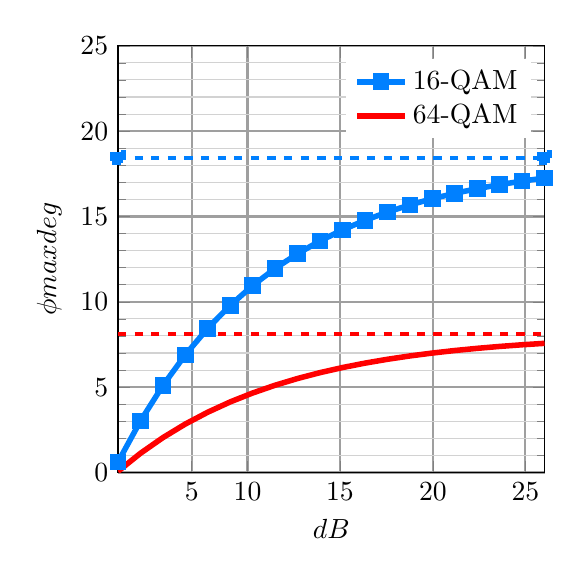
\begin{tikzpicture}[scale=1]
	\begin{semilogxaxis}[
			height			=	7cm							,
			width			=	7cm							,
			xlabel			=	{$\SNR\myunit{dB}$}			,
			ylabel			=	{$\phi\sub{max}\myunit{deg}$}			    ,
                xticklabels     =   {$5$,$10$,$15$,$20$,$25$}        ,
                xtick           =   {5,10,31.5,100,315}             ,
			xmin			=	2    						,
			xmax			=	400							,
			ymin			=	0							,
			ymax			=	25							,
			legend entries	=	{16-QAM, 64-QAM}			,
			legend style	=	{draw = none}				,
			legend pos		=	north east					,
		    grid 			=   both						,
		    minor tick num 	= 	4 							,
		    minor grid style=   {draw=gray!35} 				,
		    major grid style=   {thick,draw=gray!75} 		,
			]
			
				
		\addplot[
			mark 			= square*,
			color 			= blue!50!cyan, 
			samples 		= 20, 
			domain  		= 2:400,
			line width 		= 2pt]
			{atan((1-sqrt(2*(16-1)/16/x))/(sqrt(16)-1)};
			
		\addplot[
			mark 			= none,
			color 			= red, 
			samples 		= 20, 
			domain  		= 2:400,
			line width 		= 2pt]
			{atan((1-sqrt(2*(64-1)/64/x))/(sqrt(64)-1)};

		\addplot[
			mark 			= square*,
			color 			= blue!50!cyan, 
			samples 		= 2, 
			domain  		= 2:400,
			line width 		= 1.5pt,
			dashed]
			{atan((1/(sqrt(16)-1)};
			
		\addplot[
			mark 			= none,
			color 			= red, 
			samples 		= 2, 
			domain  		= 2:400,
			line width 		= 1.5pt,
			dashed]
			{atan((1/(sqrt(64)-1)};

	\end{semilogxaxis}
\end{tikzpicture}
